% ABOUTME: Verification: the ISS reference model, directed and random tests, counters, bugs found.
% ABOUTME: Owner: Trishit (review, add annotated waveform screenshots from GTKWave or Surfer).
\section{Verification}
\label{sec:verification}

\subsection{Method}
A test passes only if the hardware ends in exactly the state the
instruction set architecture defines. We wrote a two-pass assembler and an
instruction set simulator (ISS) in Python (\texttt{tools/rvasm.py},
\texttt{tools/iss.py}). The assembler's encodings are checked against the
RISC-V specification \cite{riscvspec} by 34 unit tests, and the ISS is checked
on hand-computed programs before anything is compared with it. One
testbench (\texttt{tb/tb\_cpu.v}) serves all three CPUs under Icarus Verilog
\cite{icarus}. It runs a program until \texttt{ecall}, then dumps all 32
registers, all 256 data words and the performance counters. The runner
(\texttt{tools/sim.py}) compares every register, every memory word and the
instruction count with the ISS. Each program runs on all three CPUs.

\subsection{Tests}
Directed tests (Table~\ref{tab:tests}) each aim at one case the pipeline can
get wrong. Five benchmarks (array sum, Fibonacci, bubble sort and two
microbenchmarks) are checked the same way. A constrained-random generator
(\texttt{tools/randprog.py}) writes 40 programs of 46 instructions over only
six registers, mixing arithmetic, loads and stores to eight shared words and
forward branches, so hazards at every distance occur far more often than in
hand-written code. Finally, four tests check the performance counters: CPI is
exactly 1 on the single-cycle CPU, (\ref{eq:cycles}) holds on every program, a
false hazard costs no cycle, and forwarding leaves no arithmetic stall.
In total the suite runs 229 checks in about three seconds and runs in
continuous integration on every pull request.

\begin{table}[t]
\centering
\caption{Directed tests}
\label{tab:tests}
\begin{tabular}{@{}lp{5.4cm}@{}}
\toprule
Program & What it catches \\
\midrule
\texttt{alu\_ops} & every ALU operation, signed compares, shift by 31 \\
\texttt{x0\_reg} & writes to x0 dropped, never forwarded \\
\texttt{raw\_hazards} & RAW at distance 1, 2 and 3 on both operands \\
\texttt{load\_use} & load then use as rs1, rs2, base address, store data \\
\texttt{store\_data} & store data and address from the previous instruction \\
\texttt{branches} & taken and not taken, operands from ALU and load, back to back \\
\texttt{halt\_shadow} & instructions after \texttt{ecall} never commit \\
\texttt{false\_hazard} & immediate bits that look like rs2 do not stall \\
\texttt{hazard\_demo} & one forward, one load-use stall, one flush \\
\bottomrule
\end{tabular}
\end{table}

\subsection{Pipeline timing}
The testbench writes the PC in every stage on every cycle. From that trace we
draw the pipeline diagram of Fig.~\ref{fig:diagram}, so the figure shows the
hardware's behaviour, not our intention. Fig.~\ref{fig:wave} shows the same
run as a waveform, read from the simulation's VCD file. The overlap of
instructions, the stall of \texttt{add x4} behind the load, the two flushed
instructions after the taken \texttt{beq}, and the forwarding selects
(EX/MEM in cycles 4, 6 and 8, MEM/WB in cycle 7) are all visible.

\begin{figure}[t]
\centering
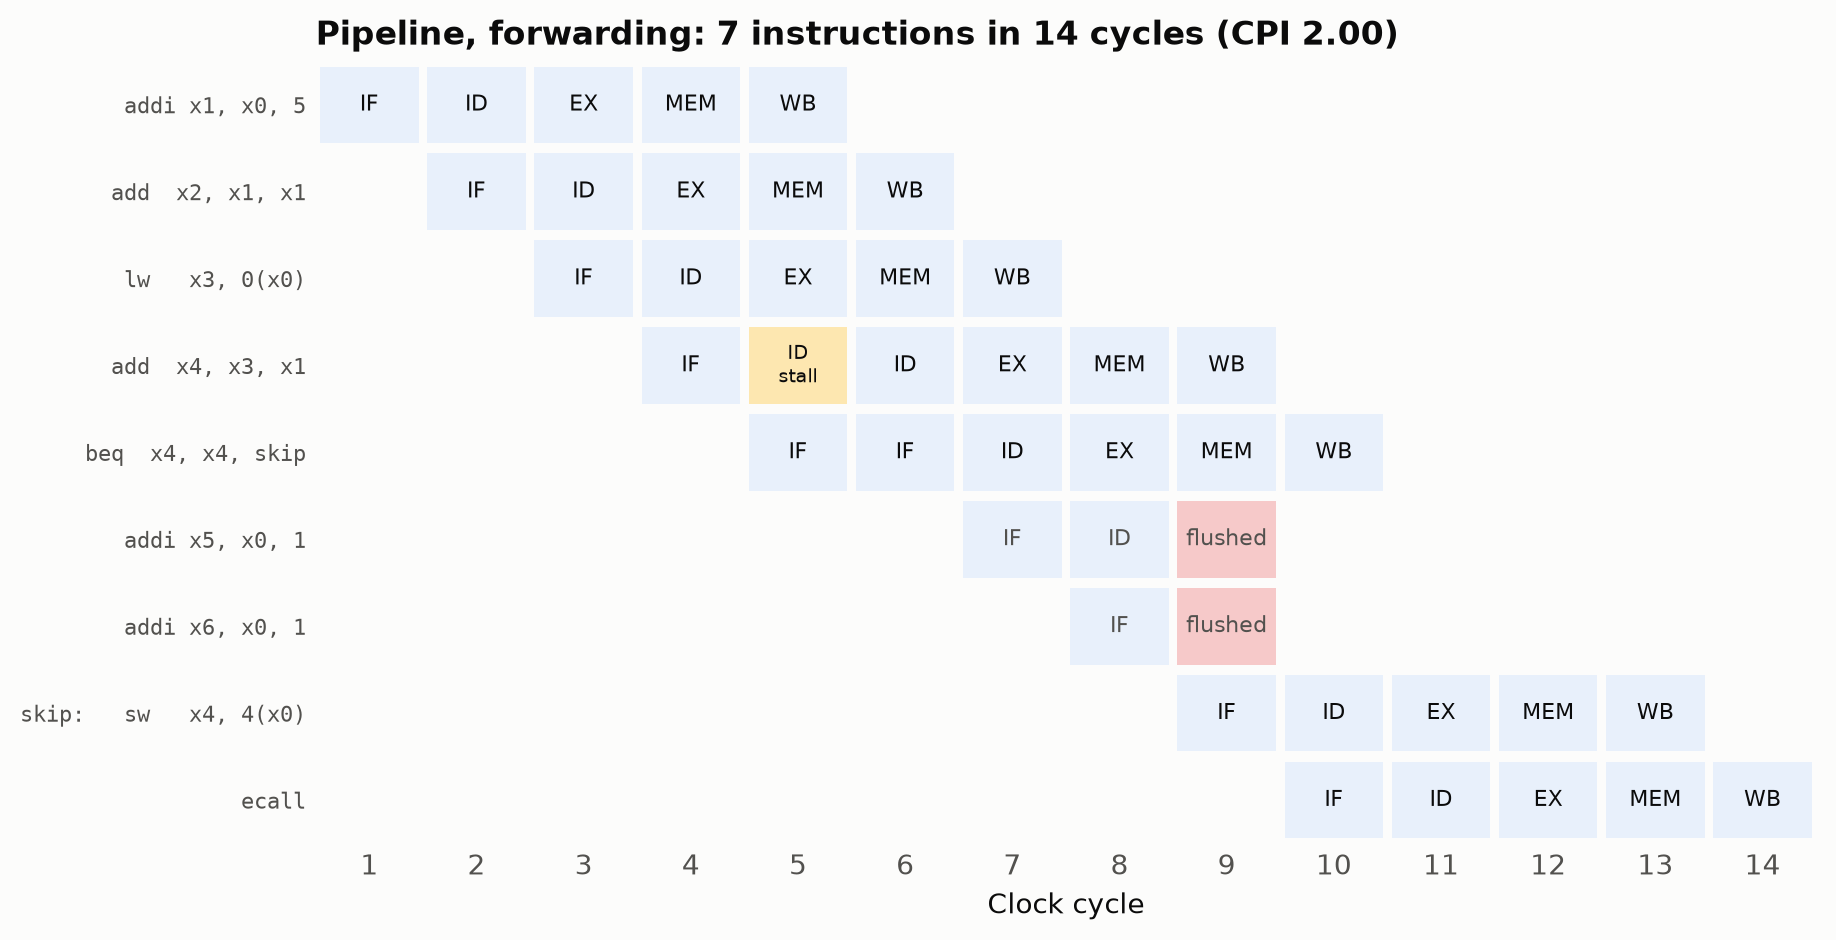
\includegraphics[width=\columnwidth]{pipeline_diagram_pipe_fwd.png}
\caption{Pipeline diagram of the hazard demo on the forwarding pipeline,
drawn from the RTL trace. Yellow: load-use stall. Red: flushed.}
\label{fig:diagram}
\end{figure}

\begin{figure}[t]
\centering
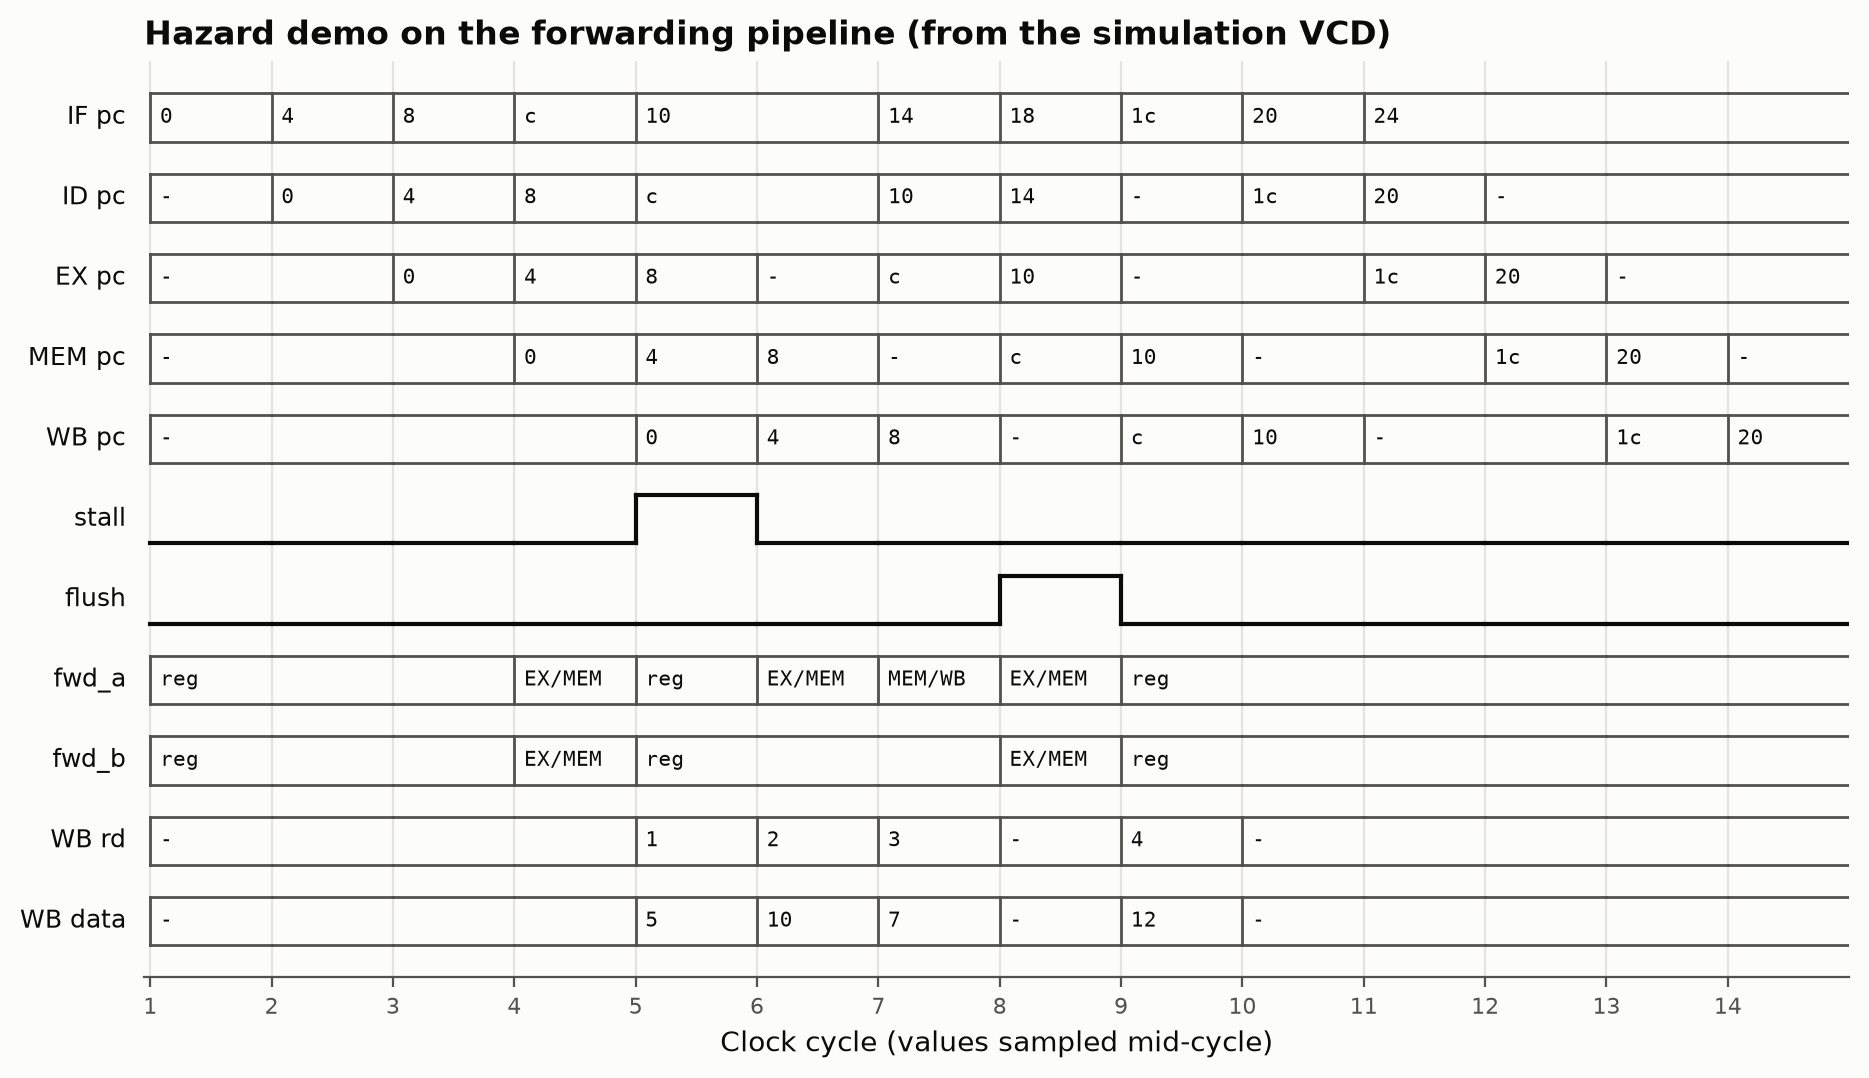
\includegraphics[width=\columnwidth]{waveform_hazard_demo.png}
\caption{Waveform of the same run: PC in each stage (\texttt{-} is a bubble),
stall, flush, forwarding selects and write back.}
\label{fig:wave}
\end{figure}

\subsection{Bugs the flow caught}
Four defects were found and fixed during development, each with its root
cause:
\begin{enumerate}
\item The forwarding and hazard logic was first written as Verilog functions
called from \texttt{assign}. Such an assignment is only re-evaluated when the
function's \emph{arguments} change, not when the module signals it reads
change, so forwarding selects went stale. The ISS comparison failed on the
first program; the logic now uses \texttt{always @(*)}.
\item With forwarding disabled, Icarus folded the constant \texttt{if
(ENABLE)} away and left an \texttt{always @(*)} block with no sensitivity,
so the selects stayed unknown. The enable now applies outside the block.
\item Synthesis of the single-cycle CPU reported a combinational loop through
the register file bypass (Section~\ref{sec:pipeline}).
\item An initial NOP fill of instruction memory took priority over the
program file in one synthesis mode, so Yosys saw a CPU that only ran NOPs and
removed it entirely. The fill now exists only in simulation.
\end{enumerate}
